{\actuality} Возможные направления применения мобильных роботов включают в себя использование их для исследовательских целей в труднодоступных условиях. Мобильные роботы могут проникать в места, недоступные и опасные для людей, например, в пещеры и шахты, перемещаться под завалами или внутри помещений во время стихийных бедствий, аварийных ситуаций и так далее. 
Одним из наиболее интересных и малоизученных направлений является разработка мобильных роботов, предназначенных для движения в условиях пещер естественного происхождения. 

Движение по пещере часто происходит по опасным и труднопроходимым участкам. Наиболее опасными являются сифоны \pic{fig:surface_types/syphon}, сталактиты, сталагмиты, обилие скользких грунтов \pic{fig:surface_types/ice, fig:surface_types/moss, fig:surface_types/clay}. В пещерах недостаток света, часто влажно. Встречаются участки, покрытые водой \pic{fig:surface_types/splash} и растительностью \pic{fig:surface_types/moss}.

\begin{figure}[H]
  \begin{subfigure}[b]{0.3\textwidth}
      \centering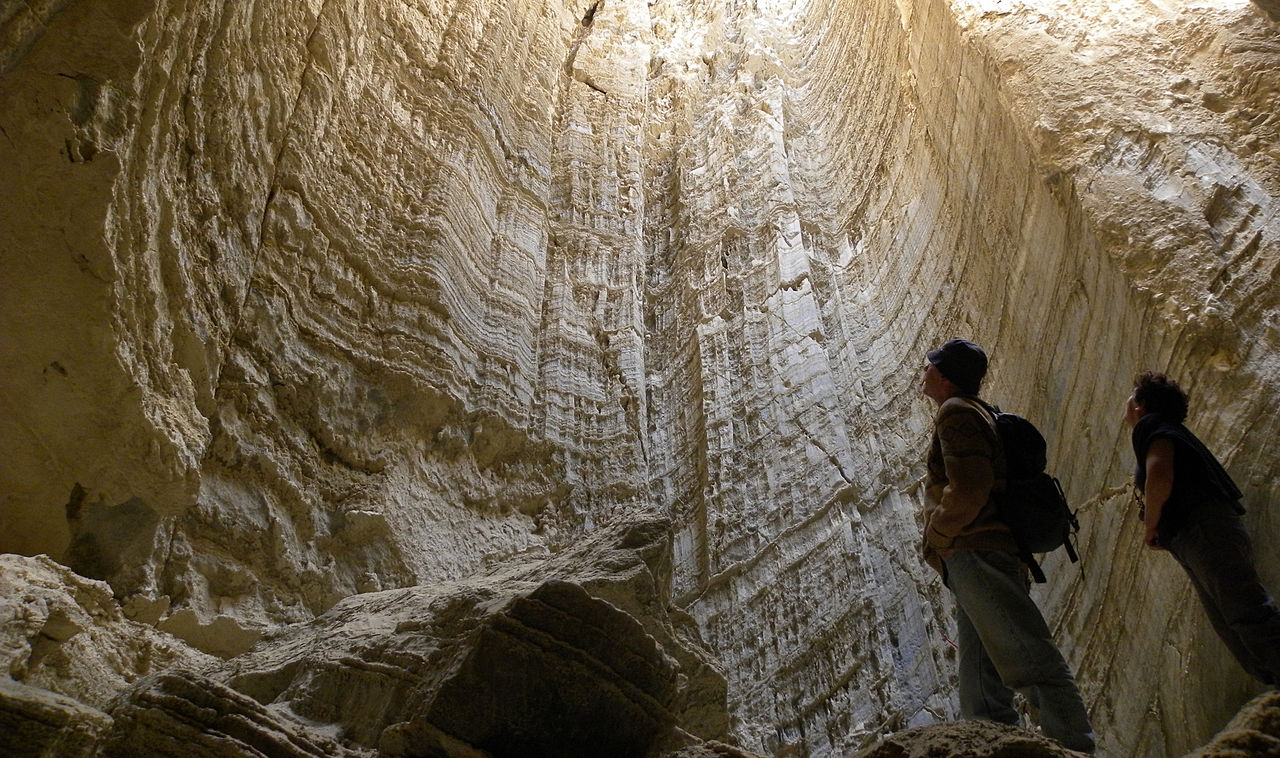
\includegraphics[height=2.8cm,width=1\textwidth,keepaspectratio]{surface_types/salt.jpg}\\
      \caption{Соляные отложения}
      \label{fig:surface_types/salt}
  \end{subfigure}
  \hfill
  \begin{subfigure}[b]{0.3\textwidth}
      \centering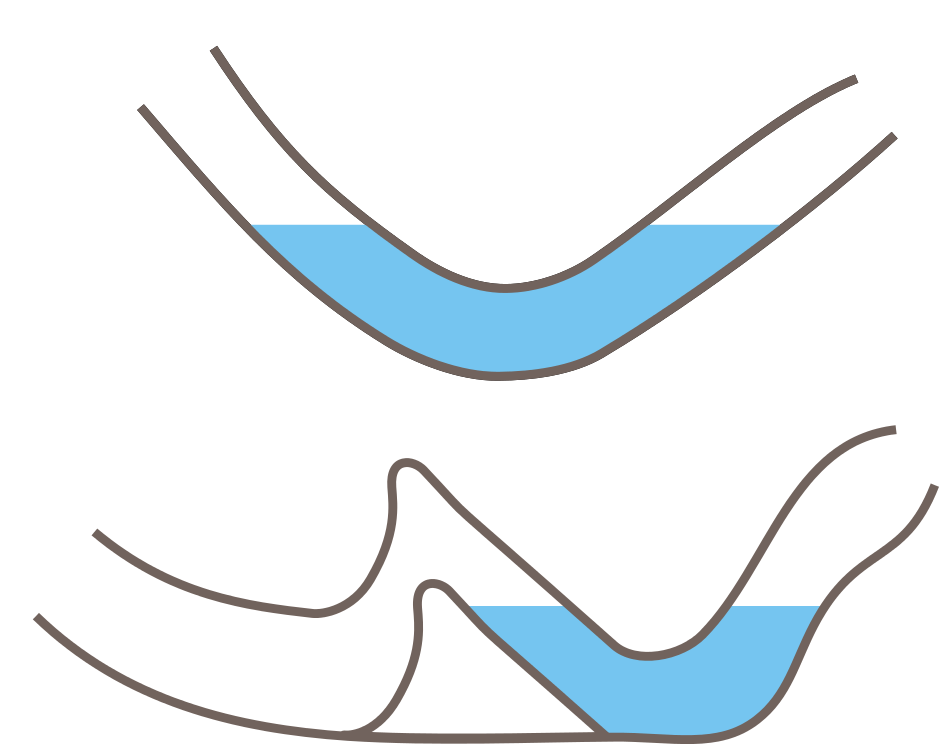
\includegraphics[height=2.8cm,width=1\textwidth,keepaspectratio]{surface_types/siphon.png}\\
      \caption{Сифон}
      \label{fig:surface_types/syphon}
  \end{subfigure}
  \hfill
  \begin{subfigure}[b]{0.3\textwidth}
      \centering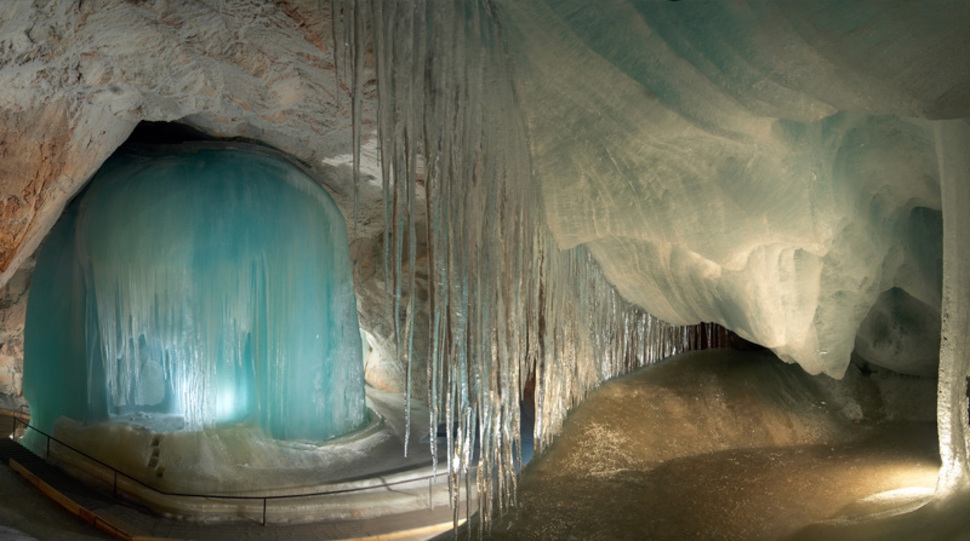
\includegraphics[height=2.8cm,width=1\textwidth,keepaspectratio]{surface_types/ice.png}\\
      \caption{Ледяная пещера}
      \label{fig:surface_types/ice}
  \end{subfigure}

  \begin{subfigure}[b]{0.3\textwidth}
      \centering
      \begin{tikzpicture}
          % Include the image in a node
          \node [above right, inner sep=0] (image) at (0,0)
          {\centering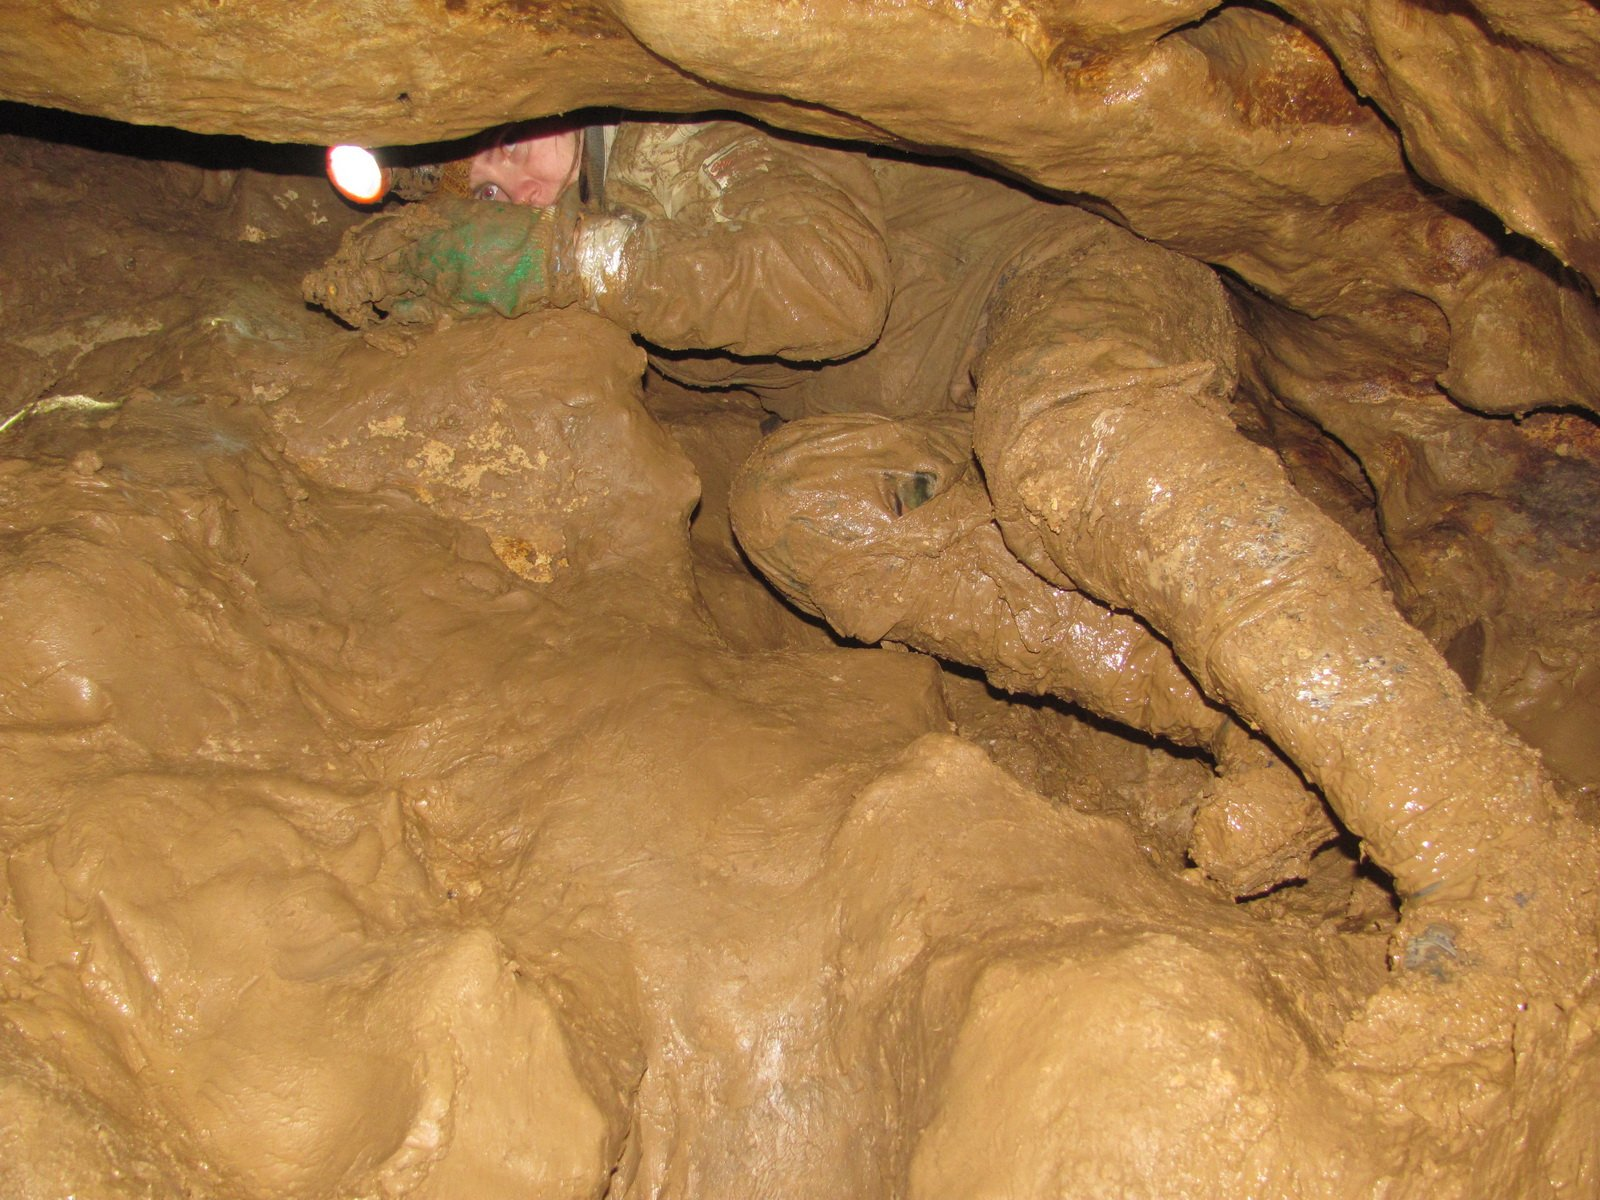
\includegraphics[height=2.8cm,width=1\textwidth,keepaspectratio]{surface_types/clay.jpg}};
          % Create scope with normalized axes
          \begin{scope}[
                  x={($ 0.1*(image.south east)$)},
                  y={($ 0.1*(image.north west)$)}]
              % Grid and axes' labels
              % \draw[lightgray,step=1] (image.south west) grid (image.north east);
              % \foreach \x in {0,1,...,10} { \node [below] at (\x,0) {\x}; }
              % \foreach \y in {0,1,...,10} { \node [left] at (0,\y) {\y};}
              % Labels
              \draw[stealth-, very thick,green] (6,8) -- ++(1,1)
              node[rounded corners=3pt,right,black,fill=white]{\tiny Человек};
          \end{scope}
      \end{tikzpicture}
      \caption{Глина}
      \label{fig:surface_types/clay}
  \end{subfigure}
  \hfill
  \begin{subfigure}[b]{0.3\textwidth}
      \centering
      \begin{tikzpicture}
          % Include the image in a node
          \node [above right, inner sep=0] (image) at (0,0)
          {\centering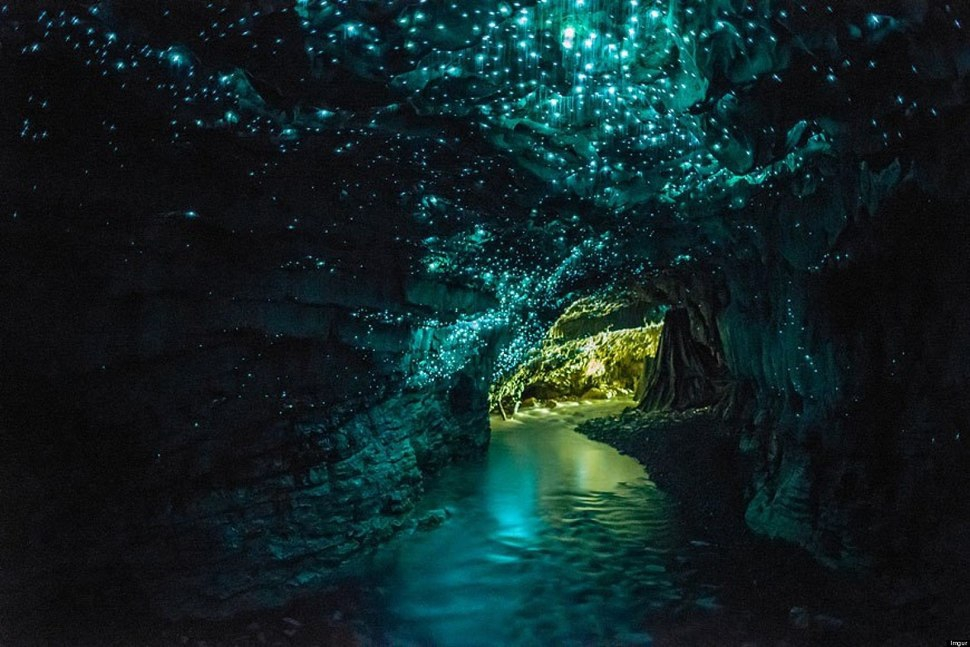
\includegraphics[height=2.8cm,width=1\textwidth,keepaspectratio]{surface_types/splash.png}};
          % Create scope with normalized axes
          \begin{scope}[
                  x={($ 0.1*(image.south east)$)},
                  y={($ 0.1*(image.north west)$)}]
              % Grid and axes' labels
              % \draw[lightgray,step=1] (image.south west) grid (image.north east);
              % \foreach \x in {0,1,...,10} { \node [below] at (\x,0) {\x}; }
              % \foreach \y in {0,1,...,10} { \node [left] at (0,\y) {\y};}

              % Labels
              \draw[stealth-, very thick,green] (5,2) -- ++(-2,+1)
              node[rounded corners=3pt,left,black,fill=white]{\tiny Лужа};
          \end{scope}
      \end{tikzpicture}
      \caption{Пещера, заполненная водой по~колено}
      \label{fig:surface_types/splash}
  \end{subfigure}
  \hfill
  \begin{subfigure}[b]{0.3\textwidth}
      \centering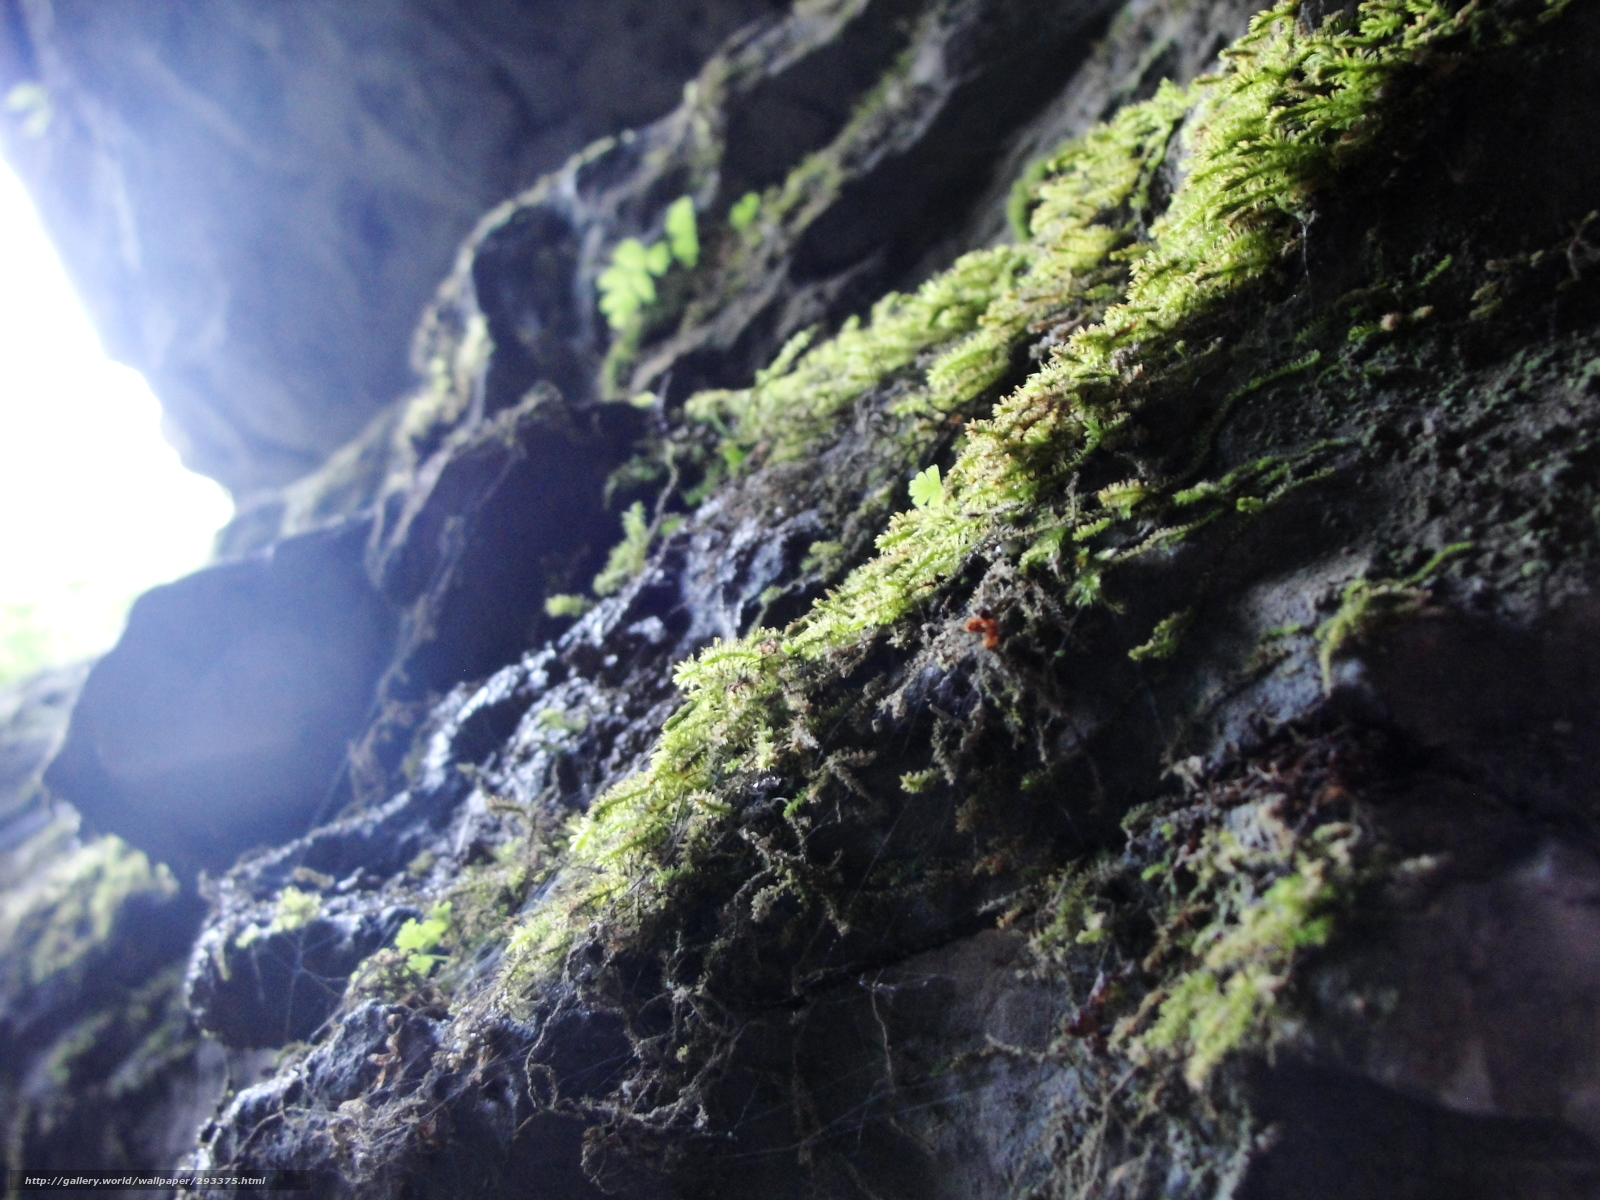
\includegraphics[height=2.8cm,width=1\textwidth,keepaspectratio]{surface_types/moss.jpg}\\
      \caption{Мох}
      \label{fig:surface_types/moss}
  \end{subfigure}
  \caption{Препятствия, встречающиеся в пещерах}\label{fig:obstacles}
\end{figure}

Эти препятствия могут встретиться человеком при исследовании или инспекции пещеры. Одно из преимуществ роботов --- они могут работать в опасных средах без нахождения рядом человека. Таким образом использование роботов в пещерах нивелирует все опасности для человека.

Существуют различные типы движителей роботов. С препятствиями, представленными выше, лучше всего справляются многоногие шагающие роботы. Такие роботы могут проходить по сыпучим грунтам, каменистым грядам и преодолевать небольшие водные преграды.

Для полноценного функционирования любого мобильного робота необходимы сенсоры. Сенсоры мобильных роботов можно разделить на внешние и внутренние. Под внешними сенсорами подразумеваются устройства, элементы которых не могут быть защищены от воздействия окружающей среды. Примерами таких сенсоров являются камеры, лидары, сонары и тому подобные устройства.

Внутренние сенсоры включают в себя датчики усилий, акселерометры, магнитометры, амперметры и так далее. Такие устройства предполагают взаимодействие с внешней средой посредством гравитационных или магнитных полей, или механических элементов, и могут быть механически защищены от неблагоприятного воздействия окружающей среды.

Большую опасность для мобильных роботов представляет тот факт, что характерные для пещеры условия могут вывести из строя сенсоры. К примеру грязь \pic{fig:surface_types/clay} может закрыть обзор камере или лидару. Или водная гладь \pic{fig:surface_types/splash} будет отражать лучи лазера лидара и искажать данные \pic{fig:unsolvable_case}.

      \begin{figure}[ht!]
      \begin{subfigure}[t]{0.3\textwidth}
        \centering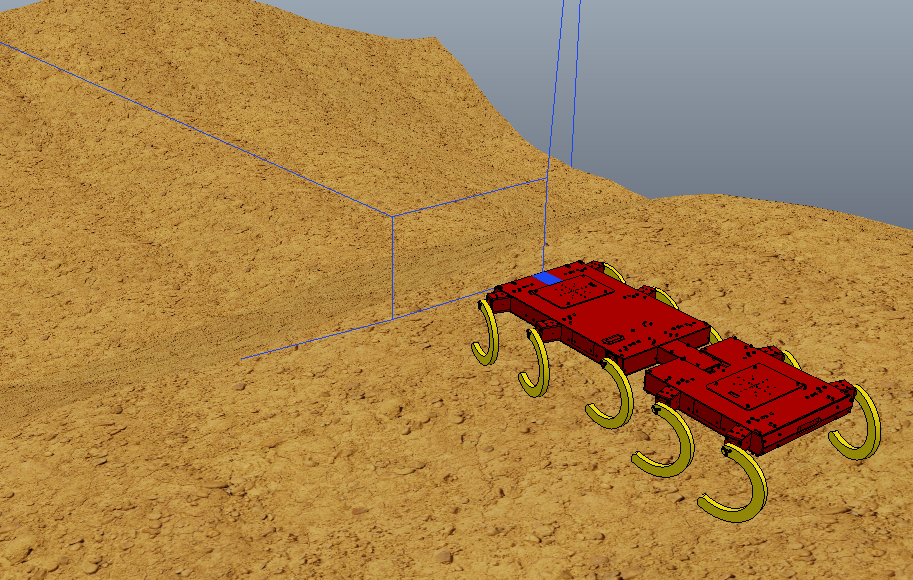
\includegraphics[height=3cm,width=1\textwidth,keepaspectratio]{terrain_wo_water.png}
        \caption{Территория без воды}
    \end{subfigure}
          \begin{subfigure}[t]{0.35\textwidth}
              \centering
              \begin{tikzpicture}
                  % Include the image in a node
                  \node [above right, inner sep=0] (image) at (0,0)
                  {\centering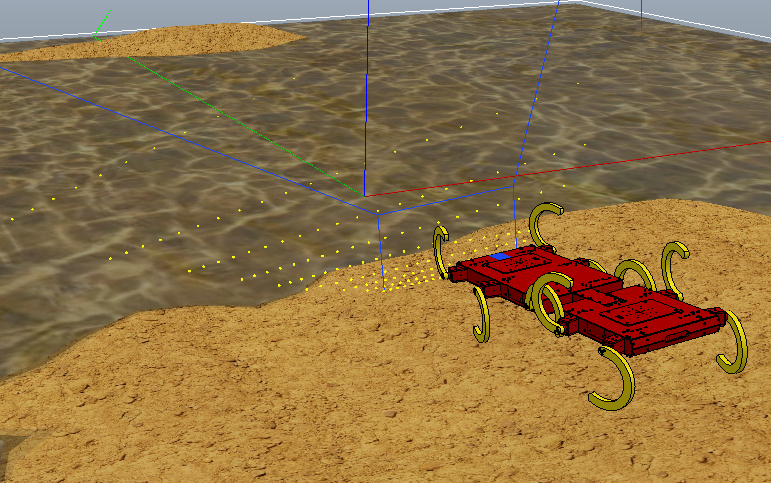
\includegraphics[height=3.5cm,width=1\textwidth,keepaspectratio]{terrain_w_water1.png}};
                  % Create scope with normalized axes
                  \begin{scope}[
                          x={($ 0.1*(image.south east)$)},
                          y={($ 0.1*(image.north west)$)}]
                      % Grid and axes' labels
                      \draw[stealth-, very thick,green] (6,8) -- ++(2,1)
                      node[rounded corners=3pt,right,black,fill=white]{\tiny Вода};

                      \draw[stealth-, very thick,green] (0.5,5.5) -- (3,2);
                      \draw[stealth-, very thick,green] (2.5,4.2) -- (3,2);
                      \draw[stealth-, very thick,green] (4.5,4) -- (3,2)
                      node[rounded corners=3pt,below,black,fill=white]{\tiny Данные с лидара};
                  \end{scope}
              \end{tikzpicture}
              \caption{Территория с водой}
              \label{fig:terrain_w_water1.png}
          \end{subfigure}
          \begin{subfigure}[t]{0.3\textwidth}
              \centering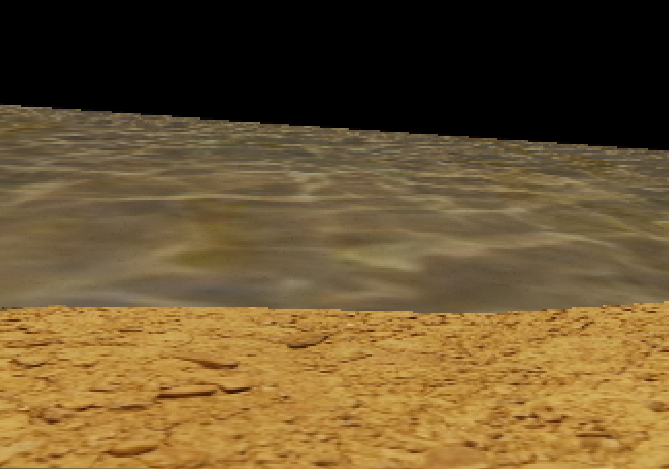
\includegraphics[height=3cm,width=1\textwidth,keepaspectratio]{terrain_w_water_camera.png}
              \caption{Изображение с камеры}
          \end{subfigure}
          \caption{Примеры ситуаций, где навигация, основанная на камере или лидаре построит неправильную карту}
          \label{fig:unsolvable_case}
      \end{figure}
  % \legend{Подрисуночный текст, описывающий обозначения, например. Согласно
  %     ГОСТ 2.105, пункт 4.3.1, располагается перед наименованием рисунка.}

% \ifsynopsis
% Этот абзац появляется только в~автореферате.
% Для формирования блоков, которые будут обрабатываться только в~автореферате,
% заведена проверка условия \verb!\!\verb!ifsynopsis!.
% Значение условия задаётся в~основном файле документа (\verb!synopsis.tex! для
% автореферата).
% \else
% Этот абзац появляется только в~диссертации.
% Через проверку условия \verb!\!\verb!ifsynopsis!, задаваемого в~основном файле
% документа (\verb!dissertation.tex! для диссертации), можно сделать новую
% команду, обеспечивающую появление цитаты в~диссертации, но~не~в~автореферате.
% \fi

{\aim} является разработка метода построения карты местности с определением геометрических и физико-механических свойств опорной поверхности роботом с шагающими движителями снабженными тактильными датчиками.

Предлагаемое решение подходит для первичного исследования замкнутых труднодоступных пространств, где отсутствует освещение, присутствует обилие грязи, пыли, а также водных препятствий. Алгоритмы и концепты навигации данной системы могут быть использованы как резервная система навигации для других робототехнических систем, когда более точная --- оптическая вышла из строя.

Для~достижения поставленной цели решаются следующие {\tasks}:
\begin{enumerate}[beginpenalty=10000] % https://tex.stackexchange.com/a/476052/104425
    \item Определение профиля опорной поверхности, на основе информации о точках её касания ногами робота и внутренних датчиков, характеризующих механическое состояние аппарата.
    \item Определение физико-механических свойств опорной поверхности: жесткости, вязкости и пластичности, и выделение на их основе классов поверхностей на основе информации с датчиков силы, установленных на ногах и внутренних датчиков робота.
    \item Исследование влияния на точность измерения усилий площади пятна контакта при нажатии на сенсор.
    \item Изучение влияния геометрических параметров робота на точность и полноту физико-механических свойств опорной поверхности и профильную проходимость робота.
\end{enumerate}

{\researchobj}
Объектом исследования является класс многоногих шагающих роботов с цельным или сочленённым корпусом, и цикловыми движителями с одной степенью свободы, управляемые зависимо или независимо друг от друга.

\begin{figure}[H]
    \centerfloat{
        \hfill
        \subcaptionbox[List-of-Figures entry]{Первая итерация\label{fig:strirus_0}}{%
            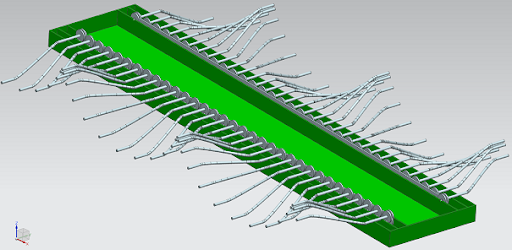
\includegraphics[width=0.33\linewidth]{strirus_0.png}}
        \hfill
        \subcaptionbox[List-of-Figures entry]{Вторая итерация \label{fig:strirus_1}}{%
            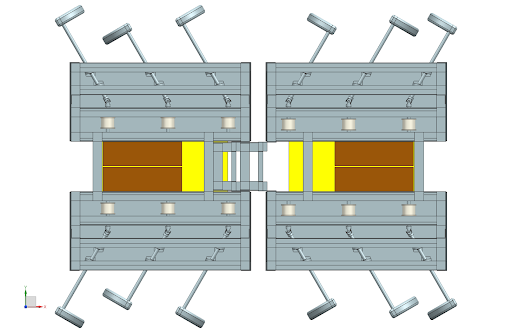
\includegraphics[width=0.33\linewidth]{strirus_1.png}}
        \hfill
        \subcaptionbox{Третья итерация\label{fig:strirus_2}}{%
        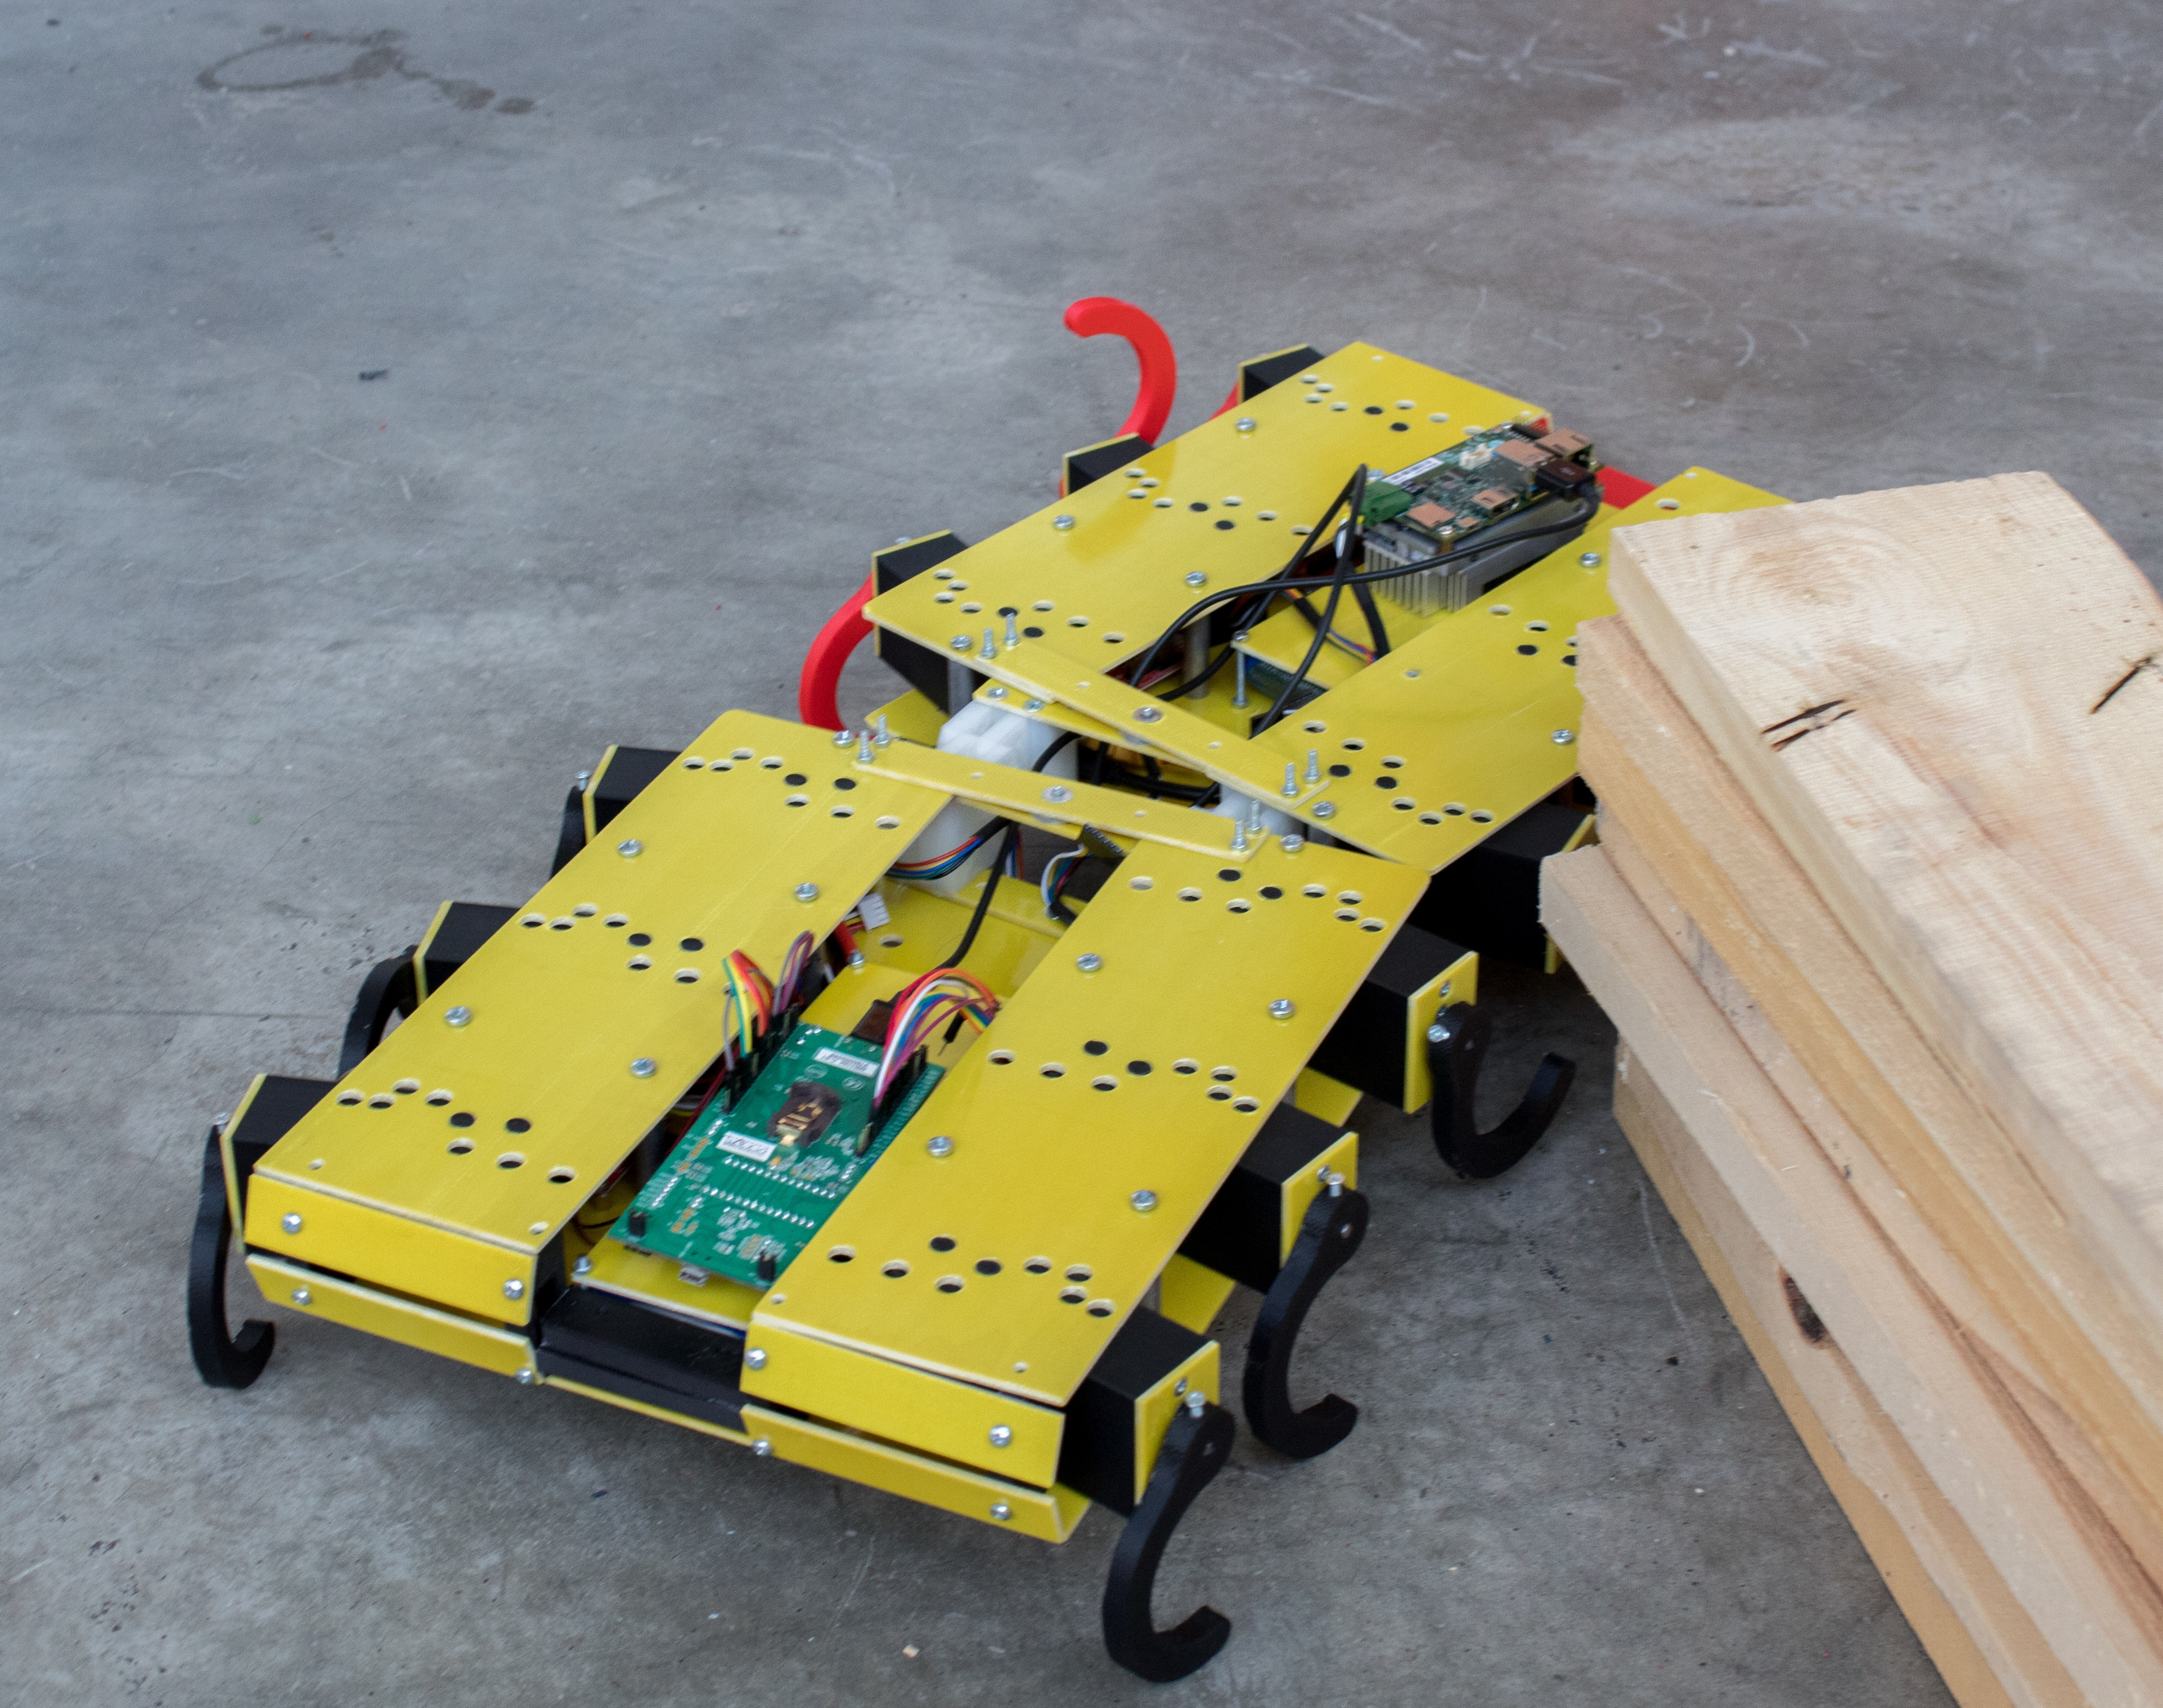
\includegraphics[width=0.33\linewidth]{strirus_2.jpg}}
        \hfill
        \subcaptionbox{Третья итерация +\label{fig:strirus_3}}{%
        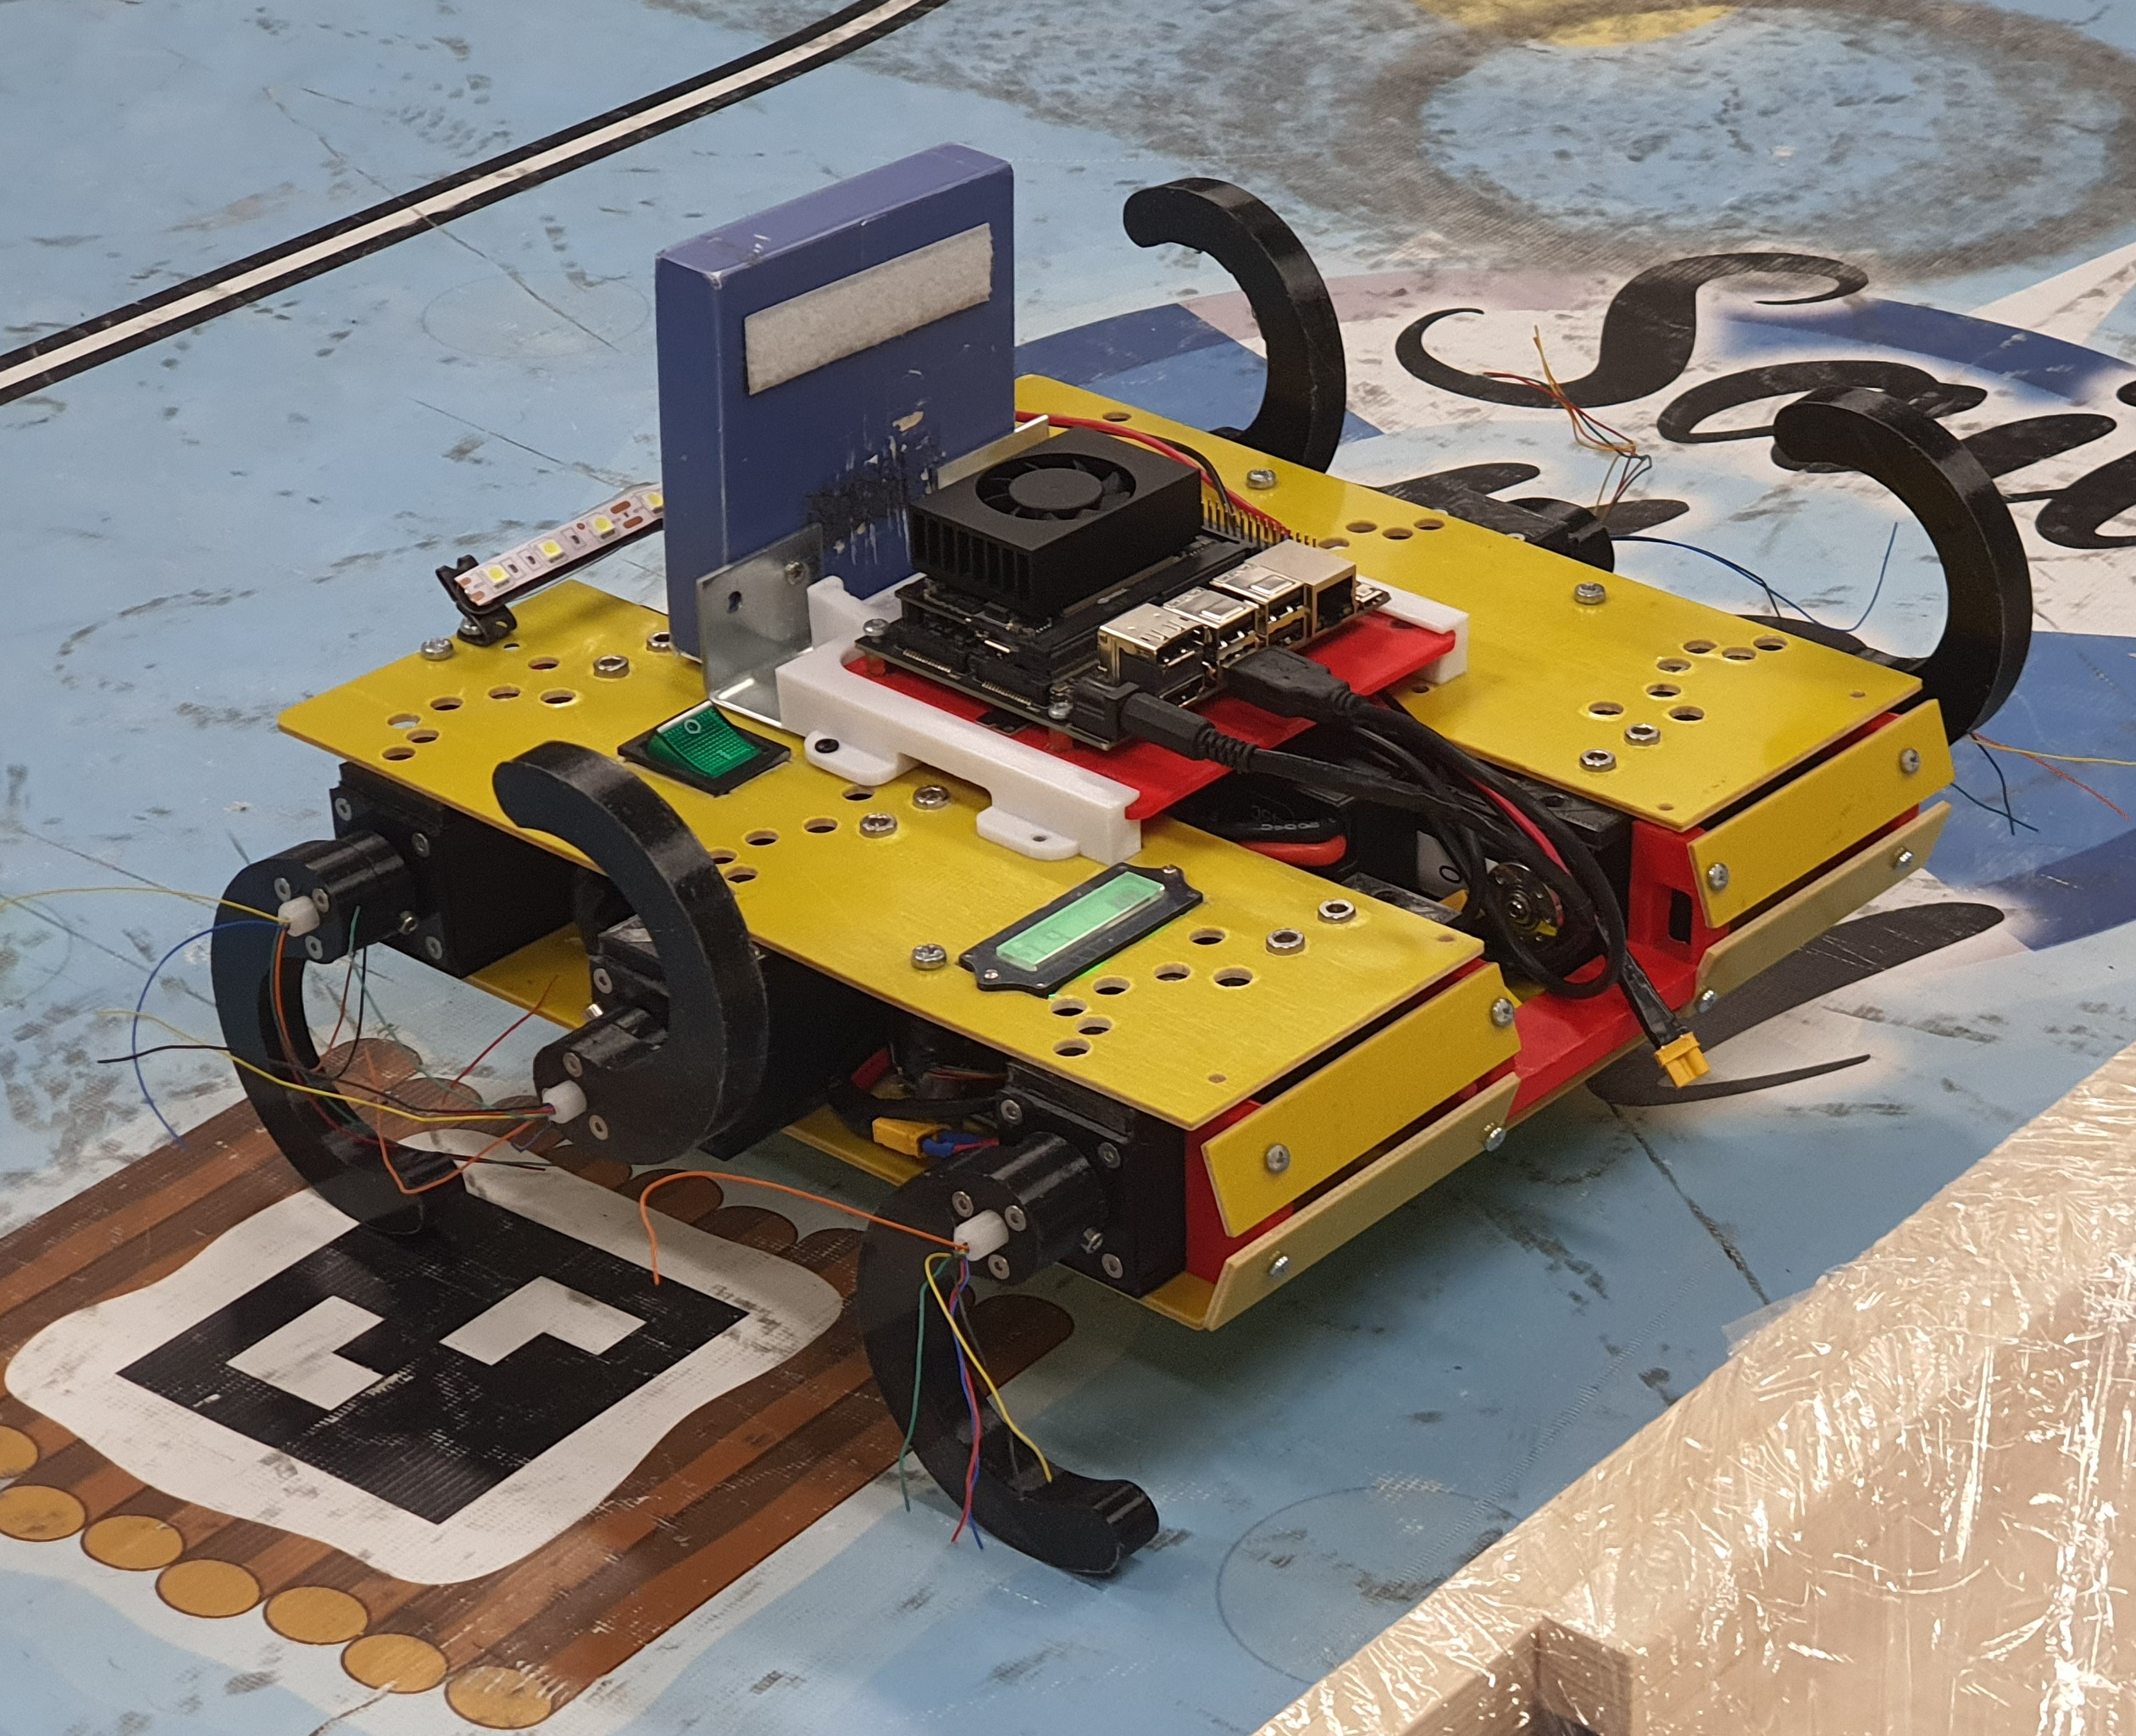
\includegraphics[width=0.35\linewidth]{strirus_3.JPG}}
        \hfill
        \subcaptionbox{Четвертая итерация\label{fig:strirus_4}}{%
        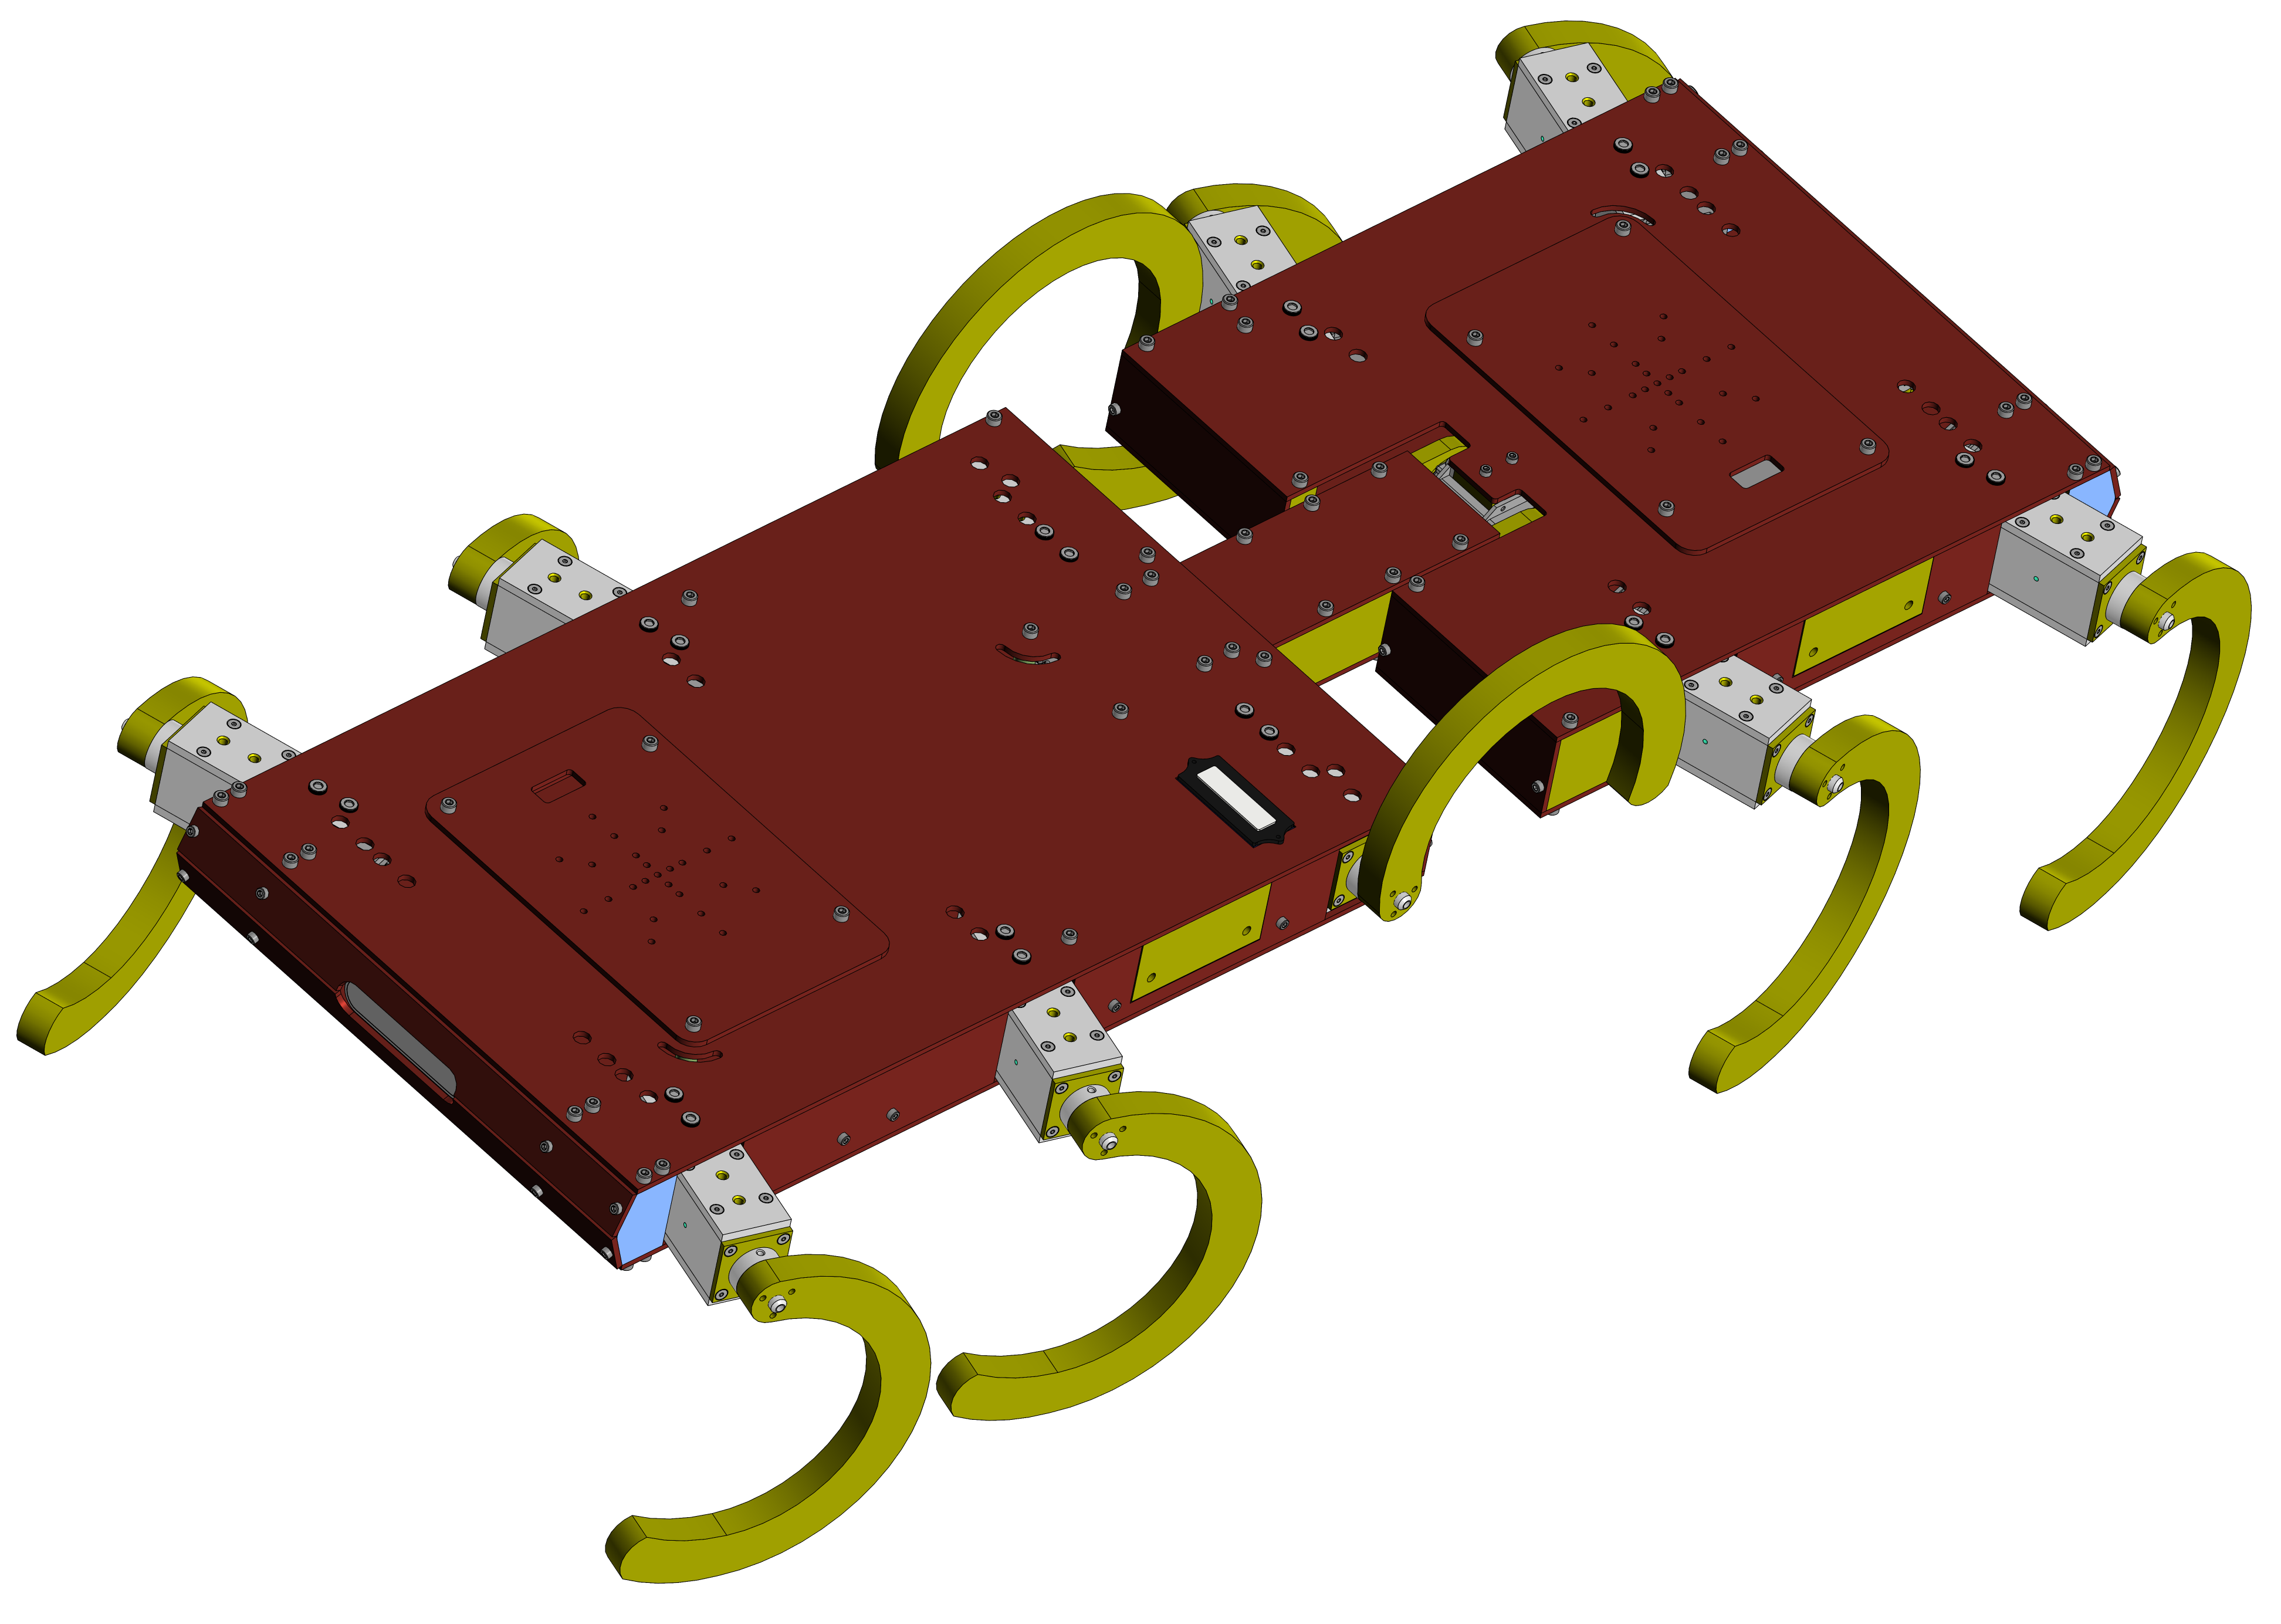
\includegraphics[width=0.35\linewidth]{strirus_4.png}}
    }
    \caption{Итерации разработанного робота СтриРус}\label{fig:striruses}
  \end{figure}

  Были разработаны ряд компьютерных и две натурных модели робота такого класса под общим названием СтриРус \pic{fig:striruses}, на базе которых проводились численные и натурные эксперименты. В процессе исследования модели уточнялись и изменялись. Так, первая модель \pic{fig:strirus_0} имела цельный корпус и настраиваемое количество ног вплоть до нескольких десятков. По результатам исследования этой модели выяснилось, что большое количество ног является излишним. Поэтому во второй модели использовалось фиксированное количество -- 12 ног, размещённых на двухсегментном корпусе, причём плоскости вращения ног расположены под углом к сагиттальной плоскости робота \pic{fig:strirus_1}. При изготовлении натурной модели робота была изменена форма ног и предусмотрены индивидуальные приводы для каждой ноги \pic{fig:strirus_2}. Часть натурных экспериментов проводилась с помощью робота с цельным корпусом \pic{fig:strirus_3}, а также на специально разработанном экспериментальном стенде. Последняя итерация модели, исправляющая выявленные недостатки предыдущих, имеет 10 увеличенных ног с независимым приводом, распределённых по двум сегментам корпуса и возможностью изменения углов между корпусом и плоскостями вращения ног \pic{fig:strirus_4}.

{\methods} За основу были взяты методологии из теории по разработке робототехнических систем, теоретической механики, механизмов и машин, теории оптимизации.

Для экспериментального исследования применялось численное, натурное и стендовое моделирование.

{\reliability} Достоверность результатов обеспечивается согласованностью с опубликованными результатами научных исследований других авторов, подтверждаются результатами компьютерного моделирования, натурными испытаниями. Результаты диссертационного исследования докладывались и обсуждались на российских и международных научных конференциях, и получили положительный отзыв научной общественности.

{\novelty} 
\begin{enumerate}
    \item Реализован метод построения карты местности, состоящий в определении геометрической формы поверхности с помощью тактильного очувствления, который позволяет решать задачу определения плана и профиля поверхности в условиях отсутствия видимости и при движении по поверхности, находящейся под водой. \textbf{Доказана} возможность построения карты местности с помощью тактильного очувствления, как в робототехническом симуляторе, так и с помощью натурного эксперимента.
    \item Реализован метод определения физико-механических свойств опорной поверхности на основе тактильного очувствления. \textbf{Показана} возможность различать материалы с упругими, жёсткими, пластичными свойствами.
    \item \textbf{Установлено} то, что датчик силы, на основе полимерного материала, обеспечивает погрешность определения силы не более 10\% при условии площади пятна контакта не менее 25\% от размера датчика, что позволяет применять датчик такого типа для тактильного очувствления мобильного робота. \textbf{Предложена} методика роботизированного исследования датчика силы.
    \item Предложен аддитивно-мультипликативный критерий оптимизации кинематической схемы многоногих шагающих роботов с цикловыми одностепенными движителями, включающий в себя показатели проходимости и покрытия опорной поверхности. На основании которого определено оптимальное количество ног для циклового движителя с одной степенью свободы.
\end{enumerate}

\textbf{Сделан вывод} об эффективности предложенных методов и методик, на основе результатов натурных испытаний.

{\defpositions}
\begin{enumerate}[beginpenalty=10000] % https://tex.stackexchange.com/a/476052/104425
    \item Метод построения карты местности, состоящий в определении геометрической формы поверхности с помощью тактильного очувствления, который позволяет решать задачу определения плана и профиля поверхности в условиях отсутствия видимости и при движении по поверхности, находящейся под водой.
    \item Метод определения физико-механических свойств опорной поверхности на основе тактильного очувствления, позволяющий различать материалы с упругими, жёсткими, пластичными свойствами.
    \item Зависимость погрешности датчика силы на основе полимерного материла от площади пятна контакта относительно размеров датчика, применяемого для тактильного очувствления мобильного робота. Методика роботизированного исследования датчика силы.
    \item Критерий оптимизации кинематической схемы многоногих шагающих роботов с цикловыми одностепенными движителями, включающий в себя показатели проходимости, покрытия опорной поверхности и её детализации. Определение на его основе габаритов и количества движителей шагающего робота.
\end{enumerate}

{\influence} Реализация полученных результатов позволит разрабатывать мобильных шагающих роботов, способных перемещаться без использования оптических сенсоров или в условиях невозможности их использования, обеспечивая построение карты местности с определением типа и свойств опорной поверхности за счёт очувствления механизмов шагания робота. 

Такие роботы могут быть востребованы для исследования естественных пещер, объектов антропогенного происхождения в условиях, когда локализация робота с помощь камер или лидаров невозможна из-за отсутствия света, наличия пыли, дыма или иных факторов, делающих невозможным применение оптических сенсорных систем.

{\probation}
Основные положения диссертации доложены и обсуждены на конференциях:
\begin{itemize}
  \item ICINCO 2017 — 14th International Conference on Informatics in Control, Automation and Robotics (Мадрид, Испания, 26-28 июля 2017);
  \item IEEE International Conference on Robotics and Biomimetics, ROBIO 2017 (Макао, Китай, 5-8 декабря 2017);
  \item  Международная научно-практическая конференция «Прогресс транспортных средств и систем» (г. Волгоград, 9-11 октября 2018 г.);
  \item 23rd IEEE FRUCT Conference (Болонья, Италия, 13-16 ноября 2018);
  \item XXXI международная конференция молодых ученых и студентов МИКМУС-2019 (Москва, 4-6 декабря 2019 г.);
  \item Международная конференция «Зимняя Школа Робототехники в Сириусе — 2022» (Адлер, Россия, 25 января - 6 февраля 2022).
\end{itemize}

{\contribution} Все научные результаты диссертации, выдвигаемые для защиты, получены автором лично. Автор самостоятельно проводил анализ литературы по теме, участвовал в обсуждении постановки цели диссертации, лично планировал и проводил компьютерные эксперименты и физические эксперименты, спроектировал и собрал экспериментальные установки. Автор лично получил все представленные в работе численные данные. 

{%%% Реализация пакетом biblatex через движок biber
\begin{refsection}[bl-author, bl-registered]
    % Это refsection=1.
    % Процитированные здесь работы:
    %  * подсчитываются, для автоматического составления фразы "Основные результаты ..."
    %  * попадают в авторскую библиографию, при usefootcite==0 и стиле `\insertbiblioauthor` или `\insertbiblioauthorgrouped`
    %  * нумеруются там в зависимости от порядка команд `\printbibliography` в этом разделе.
    %  * при использовании `\insertbiblioauthorgrouped`, порядок команд `\printbibliography` в нём должен быть тем же (см. biblio/biblatex.tex)
    %
    % Невидимый библиографический список для подсчёта количества публикаций:

    \nocite{*}

    \printbibliography[heading=nobibheading, section=1, env=countauthorvak,          keyword=biblioauthorvak]%
    \printbibliography[heading=nobibheading, section=1, env=countauthorwos,          keyword=biblioauthorwos]%
    \printbibliography[heading=nobibheading, section=1, env=countauthorscopus,       keyword=biblioauthorscopus]%
    \printbibliography[heading=nobibheading, section=1, env=countauthorconf,         keyword=biblioauthorconf]%
    \printbibliography[heading=nobibheading, section=1, env=countauthorother,        keyword=biblioauthorother]%
    \printbibliography[heading=nobibheading, section=1, env=countregistered,         keyword=biblioregistered]%
    \printbibliography[heading=nobibheading, section=1, env=countauthorpatent,       keyword=biblioauthorpatent]%
    \printbibliography[heading=nobibheading, section=1, env=countauthorprogram,      keyword=biblioauthorprogram]%
    \printbibliography[heading=nobibheading, section=1, env=countauthor,             keyword=biblioauthor]%
    \printbibliography[heading=nobibheading, section=1, env=countauthorvakscopuswos, filter=vakscopuswos]%
    \printbibliography[heading=nobibheading, section=1, env=countauthorscopuswos,    filter=scopuswos]%
    %
    %
    %
    % ~\arabic{citeauthor} вместо 18
    {\publications} Основные результаты по теме диссертации изложены в 18~печатных изданиях,
    \arabic{citeauthorvak} из которых изданы в журналах, рекомендованных ВАК\sloppy%
    \ifnum \value{citeauthorscopuswos}>0%
        , \arabic{citeauthorscopuswos} "--- в~периодических научных журналах, индексируемых Web of~Science и Scopus\sloppy%
    \fi%
    \ifnum \value{citeauthorconf}>0%
        , \arabic{citeauthorconf} "--- в~тезисах докладов.
    \else%
    ,
    \fi%
    \ifnum \value{citeregistered}=1%
        \ifnum \value{citeauthorpatent}=1%
            Зарегистрирован \arabic{citeauthorpatent} патент.
        \fi%
        \ifnum \value{citeauthorprogram}=1%
            Зарегистрирована \arabic{citeauthorprogram} программа для ЭВМ.
        \fi%
    \fi%
    \ifnum \value{citeregistered}>1%
        зарегистрированы\ %
        \ifnum \value{citeauthorpatent}>0%
        \formbytotal{citeauthorpatent}{патент}{}{а}{}\sloppy%
        \ifnum \value{citeauthorprogram}=0 . \else \ и~\fi%
        \fi%
        \ifnum \value{citeauthorprogram}>0%
        \formbytotal{citeauthorprogram}{программ}{а}{ы}{} для ЭВМ.
        \fi%
    \fi%
    % К публикациям, в которых излагаются основные научные результаты диссертации на соискание учёной
    % степени, в рецензируемых изданиях приравниваются патенты на изобретения, патенты (свидетельства) на
    % полезную модель, патенты на промышленный образец, патенты на селекционные достижения, свидетельства
    % на программу для электронных вычислительных машин, базу данных, топологию интегральных микросхем,
    % зарегистрированные в установленном порядке.(в ред. Постановления Правительства РФ от 21.04.2016 N 335)
\end{refsection}%
% \begin{refsection}[bl-author, bl-registered]
%     % Это refsection=2.
%     % Процитированные здесь работы:
%     %  * попадают в авторскую библиографию, при usefootcite==0 и стиле `\insertbiblioauthorimportant`.
%     %  * ни на что не влияют в противном случае
%     % \nocite{vakbib2}%vak
%     % \nocite{patbib1}%patent
%     % \nocite{progbib1}%program
%     % \nocite{bib1}%other
%     % \nocite{confbib1}%conf
% \end{refsection}%
    %
    % Всё, что вне этих двух refsection, это refsection=0,
    %  * для диссертации - это нормальные ссылки, попадающие в обычную библиографию
    %  * для автореферата:
    %     * при usefootcite==0, ссылка корректно сработает только для источника из `external.bib`. Для своих работ --- напечатает "[0]" (и даже Warning не вылезет).
    %     * при usefootcite==1, ссылка сработает нормально. В авторской библиографии будут только процитированные в refsection=0 работы.
}

Диссертационная работа была выполнена при поддержке грантов:
\begin{itemize}
    \item НТИ по поддержке Центра <<Технологии компонентов робототехники и мехатроники>> на базе Университета Иннополис по теме <<Разработка роботизированных платформ для автономной подземной и наземной инспекции местности в условиях трудной проходимости и плохой видимости>>. 
    \item РФФИ № 20-38-90265 по теме <<Разработка метода очувствления мобильного шагающего робота, перемещающегося в закрытом пространстве естественного происхождения>>.
\end{itemize}

% Объем и структура находятся в файле introduction

